%!TEX TS-program = xelatex
%!TEX root = ../../maxwell2018thesis.tex

\chapter[Operationalised Stopping Strategies]{Operationalised\\Stopping Strategies}\label{chap:strategies}
In Section~\ref{sec:stopping_background:heuristics}, we discussed a number of different \emph{stopping heuristics} that have been previously defined in the literature. In this chapter, we take a number of these stopping heuristics forward to produce a series of different \emph{stopping strategies,} providing an answer that addresses \blueboxbold{HL-RQ2}.\footnote{Refer to Section~\ref{sec:intro:rqs} on page~\pageref{sec:intro:rqs} for the definition of the research question.}

\begin{figure}[h]
    \centering
    \vspace{4mm}
    \resizebox{1\hsize}{!}{
    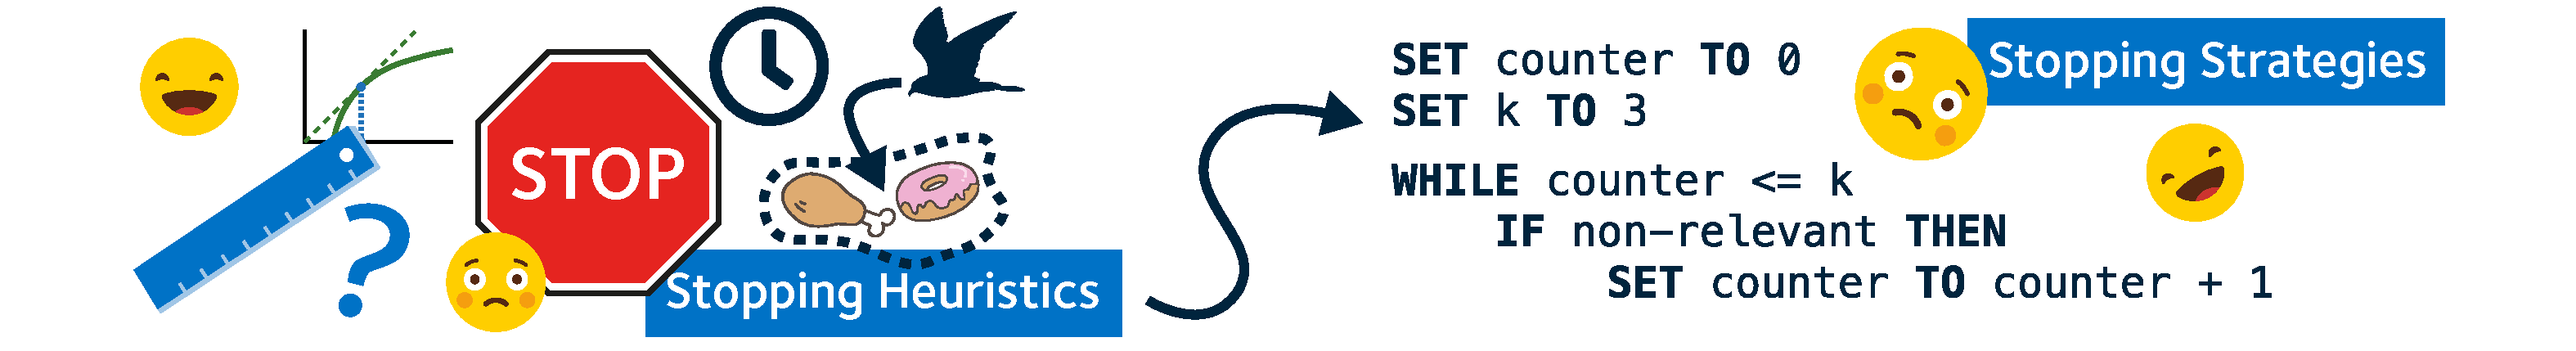
\includegraphics{figures/ch5-conversion.pdf}}
    \label{fig:conversion}
    \vspace{-5mm}
\end{figure}

These stopping strategies are operationalised versions of the corresponding heuristics. This means that we can subsequently implement and evaluate their effectiveness. We consider seven different categories of stopping strategies, which are listed below.

\begin{itemize}
    \item{\blueboxbold{Fixed Depth} blah}
    \item{\blueboxbold{Frustration} blah}
    \item{\blueboxbold{Satisfaction} blah}
    \item{\blueboxbold{Difference} blah}
    \item{\blueboxbold{\gls{acr:ift}} blah}
    \item{\blueboxbold{Time-Based} blah}
    \item{\blueboxbold{Measure-Based} blah}
\end{itemize}

\section{Fixed Depth}

\section{Frustration and Satisfaction}

\subsection{Searcher Frustration}

\subsection{Goal/Satisfaction-Based}

\subsection{Combining Frustration and Satisfaction}

\section{Difference Threshold}

\section{Instantaneous Intake}

\section{Time-Based}

\section{Measure-Based}

\section{Chapter Summary}